\chapter{性能向导}
这个向导包含了一些很好的实践来优化你的TensorFlow代码。向导被分成下面的章节:
\begin{itemize}
\item 一般的最佳实践包括常用的多种模型和硬件
\item 优化GPU详细的技巧和GPU有关
\item CPU优化 详细的CPU特定信息
\end{itemize}
\subsection{一般的最佳实践}
最佳的实践包括下面章节:
\begin{itemize}
	\item 输入pipline优化
	\item 数据格式
	\item 常用的融合操作
	\item 从源代码构建和安装
\end{itemize}
\subsubsection{输入pipeline优化}
常用的模型从磁盘获取数据在通过网络发送数据之前提前处理它,例如模型按照下面处理JPEG图像:从磁盘载入图像,解码JPEG为tensor,剪切填充,可能还有翻转和扭曲,然后分批处理。下面的图是输入pipeline。正如GPU和其它的硬件极速器会更快,预处理数据可能成为一个瓶颈。如果输入pipeline是瓶颈可能变得很复杂。一个直接的方法是在输入pipeline后减少模型为单个操作,每秒测量样本。如果对于完整的模型和单个的模型没表中样本的差别很小不同的,输入pipeline可能是瓶颈。下面有一些其它的方法识别这个问题。
\begin{itemize}
	\item 通过\lstinline[language=Bash]{watch -n 2 nvidia-smi}检查GPU是否被完全使用。如果GPU利用没有达到80-100\%,输入pipeline可能是瓶颈。
	\item 生成时间线查看大模块空白。一个生成时间线的例子在\href{https://www.tensorflow.org/performance/xla/jit}{XLA JIT}
	\item 检查CPU使用。他可能有一个优化的pipeline和缺乏CPU循环处理pipeline
	\item 评估生产力需要和验证在这个生产力条件下磁盘使用。一些云方案有网络添加磁盘速度50MB/sec,这比机械硬盘的150/MS/sec和SATA SSD的500MB/sec,PCIe SSD的2000+
 MB/sec低得多\end{itemize}
 \subsubsection{在CPU上处理}
 防止输入pipeline在CPU上能极大地提高性能。利用CPU处理输入pipeline,GPU训练。确保预处理在CPU上,按照如下操作打包:
 \begin{lstlisting}[language=Python]
 with tf.device('/cpu:0'):
     # function to get and process images or data.
     distorted_inputs = load_and_distort_images()
 \end{lstlisting}
 如果你用tf.estimator.Estimator输入函数自动放置到CPU上。
 \subsubsection{用Dataset API}
 \href{https://www.tensorflow.org/programmers_guide/datasets}{Dataset API}防止queue\_runner作为推荐的API建立输入pipelines,这个API在TensorFlow 1.2被天际到contrib中之后将被移动到TensorFlow核心。\href{https://github.com/tensorflow/models/blob/master/tutorials/image/cifar10_estimator/cifar10_main.py}{ResNet example}(\href{https://arxiv.org/pdf/1512.03385.pdf}{arXiv:1512.03385})训练CIFAR-10说明通过tf.estimator.Estimator使用Dataset API。Dataset API用C++多线程和一些低层调用而不是限制Python多线程性能的queue\_runner。尽管用feed\_dict输入数据提供了恒高的灵活性,在多数实例中feed\_dict不能规模化的优化。然而,在单个GPU上的实例使用差别可能微不足道。用Dataset API是强雷推荐的,尝试下面的代码:
 \begin{lstlisting}[language=Python]
 # feed_dict often results in suboptimal performance when using large inputs.
sess.run(train_step, feed_dict={x: batch_xs, y_: batch_ys})
 \end{lstlisting}
 \subsubsection{用大文件}
 读大量的小文件会极大地影响I/O的性能。一个方法是通过处理输入数据为(大约100MB或者更大)的TFRecord文件得到最大得到最大的I/O性能。对于小型数据集(200MB-1GB),最好的方法是载入整个数据集到内存。文档\href{https://github.com/tensorflow/models/tree/master/slim#Data}{ Downloading and converting to TFRecord format}包含一些创建TFRecord和转化CIFAR-10数据集为TFRecords的信息。
 \subsection{数据格式}
 数据格式涉及到传给Op的Tensor的结构。下面的讨论明确4D Tensor代表图像,在TensorFlow中4维Tensor的各个部分分别代表如下:
 \begin{itemize}
 	\item N:图象的批数
 	\item H:图象的高
 	\item W:代表凸显的宽
 	\item C:代表图象的通道数,1代表黑白图像,3代表真彩图像
 \end{itemize}
 在TensorFlow中有两种命名惯例,代表两种常用的格式:
 \begin{itemize}
 	\item NCHW或者channels\_first
 	\item NHWC或者channels\_last
 \end{itemize}
 NHWC是TensorFlow默认的,NCHW是在NVIDIA GPU上用cuDNN优化后的格式。构建模块的最佳实践是结合两种格式。最简单的是在GPUs上训练然后在CPUs上推理。如果TensorFLow结合\href{https://www.tensorflow.org/performance/performance_guide#tensorflow_with_intel_mkl_dnn}{Intel MKL}优化编译的,一些操作,特别是和基于CNN模型的将被优化支持NCHW。如果不用MKL,用NCHW时一些在操作将不支持在CPU上运行。
 \subsubsection{常见的融合操作}
 融合操作结合多个操作为一个内核提高性能,在TensorFlow有一些融合操作和CLA可能提高性能时创建融合操作。下面被选择的融合操作可能极大地提高性能叶东旭被忽视。
 \subsubsection{融合批规范}
 融合批规范结合多个需要批正规化的操作为一个内核。批规范对那些建立大的操作时间的比例是一个高昂的操作。用融合规范可能导致12\%-30\%的加速。有两个常见的批操作支持融合。核心tf.layers.batch\_normalization在TensorFlow 1.3 开始添加融合
 \begin{lstlisting}[language=Python]
 bn = tf.layers.batch_normallization(input_layer,fused=True,data_format = 'NCHW')
 \end{lstlisting}
 contrib中的tf.contrib.layers.batch\_norm方法从TensorFlow1.0起也有融合选项
 \begin{lstlisting}[language=Python]
 bn = tf.contrib.layers.batch_norm(input_layer, fused=True, data_format='NCHW
 \end{lstlisting}
\subsection{从源代码构建安装}
默认TensorFlow二进制针对最广泛的硬件使得TensorFlow对于每个人都可以使用。如果用CPU进行训练或者推理,推荐结合对于使用的CPU可用的优化去编译CPU。在CPU上加速推理和训练在\href{https://www.tensorflow.org/performance/performance_guide#comparing_compiler_optimizations}{Comparing compiler}被记录。

安装优化后的TensorFlow版本,从源代码\href{Comparing compiler}{构建安装},如果有在不同的硬件平台上构建TensorFlow的需要,交叉编译对于目标平台有最高的优化。下面没了是一个用bazel为指定平台编译的例子:
\begin{lstlisting}[language=Python]
# This command optimizes for Intel’s Broadwell processor
bazel build -c opt --copt=-march="broadwell" --config=cuda //tensorflow/tools/pip_package:build_pip_package
\end{lstlisting}
\subsubsection{环境构建和安装技巧}
\begin{itemize}
	\item ./configure 要求计算兼容性在构建的时候被包含。着不影响总体性能但是影响初始化启动。在运行TensorFLow一次以后,编译的内核荣光CUDA缓存。如果用一个docker容器,数据不缓存每次TensorFlow启动时间较长。通过GPUs的最佳实践是包含\href{http://developer.nvidia.com/cuda-gpus}{compute capabilities},李如意P100:6.0,Titan X(Pascal):6.1,Titan X(Maxwell):5.2和k80:3.7。
	\item 用支持所有的目标CPU优化的gcc编译器。推荐最小的gcc版本是4.8.3。在OS X上升级最新的Xcode版本用clang版本结合Xcode。
	\item 安装TensorFlow支持的最新的稳定CUDA平台和cuDNN库。
\end{itemize}
\subsubsection{优化GPU}
这部分包含指定GPU的没有在\href{https://www.tensorflow.org/performance/performance_guide#general_best_practices}{ General best practices}被包含的技巧。在多个GPU上获取优化性能是一个挑战。一个常见的方法是数据并行。通过使用数据并行利用创建多个模型的拷贝,这些模型作为一个tower,放置一个tower在每个GPU上。每个tower在不同的小批数据上操作每个tower得到更新的变量和梯度对性能有什么影响,方法,模型的收敛。下面提供了一个在多个GPUs上放置变量和tower的概览。在下一章将详细的讨论更多用于在tower分享和更新变量复杂的方法。

最好的处理变量更新的方法是依赖模型,甚至是硬件被如何配置。一个例子是一个例子是两个系统都有NVIDIA Tesla P100s一个是用PCIe另一个用\href{http://www.nvidia.com/object/nvlink.html}{NVLink}在这种场景下对于每个系统的优化方案也许不同。对于真实世界的例子,读\href{https://www.tensorflow.org/performance/benchmarks}{benchmark}详细的设置多平台优化。下面是一个benchmark多平台和配置的总结:
\begin{itemize}
	\item Tesla K80:如果GPU在相同的PCI中线跟复杂能够用\href{https://developer.nvidia.com/gpudirect}{NVIDIA GPUDirect}Peer to Peer,然后然后放置多个相等的GPUs用于训练是最好的方法。如果GPUs不能用GPUDirect,然后放置变量在CPU上是最好的选择。
	\item Titan X(Maxwell 和Pascal),M40,P100和类似的:详细的像ResNet和InceptionV,放置变量在CPU上是优化设置,但是对于有很多变量的模型像AlexNet和VGG,用GPUs和NCCL是更好。
\end{itemize}
一场用的管理变量放置的方法是创建一个方法决定每个操作放置在哪里和通过tf.device()用方法指定设备名字。考虑一个场景是一个模型在两个GPU上训练变量被放在CPU上。则将在每个GPU上循环创建放置tower,一个习惯的设备放置方法将创建监视查看操作的Variable,VariableV2和VarHanddleOp的类型,遗失者他们被放在CPU上。所有的其他操作将放在目标GPU上,构件图将按照下面处理:
\begin{itemize}
	\item 第一次循环模型中的一个tower将为gpu:0创建。当值操作期间,通常设备防治方法将指示变量被昂在cpu:0上其他操作放在gpu:0上。
	\item 第二次循环,resue设置为True预示着变量被重用tower被放置在cpu:0上被重用所有的其他操作将被创建放置在gpu:1上
\end{itemize}
最后的结果是所有的变量放在CPU上每个GPU结合模型拷贝计算操作。下面的代码段说明两个不同的变量防治方法:一个放置变量在CPU上,一个放置变量通过GPUs。
\begin{lstlisting}[language=Python]
class GpuParamServerDeviceSetter(object):
  """Used with tf.device() to place variables on the least loaded GPU.

    A common use for this class is to pass a list of GPU devices, e.g. ['gpu:0',
    'gpu:1','gpu:2'], as ps_devices.  When each variable is placed, it will be
    placed on the least loaded gpu. All other Ops, which will be the computation
    Ops, will be placed on the worker_device.
  """

  def __init__(self, worker_device, ps_devices):
    """Initializer for GpuParamServerDeviceSetter.
    Args:
      worker_device: the device to use for computation Ops.
      ps_devices: a list of devices to use for Variable Ops. Each variable is
      assigned to the least loaded device.
    """
    self.ps_devices = ps_devices
    self.worker_device = worker_device
    self.ps_sizes = [0] * len(self.ps_devices)

  def __call__(self, op):
    if op.device:
      return op.device
    if op.type not in ['Variable', 'VariableV2', 'VarHandleOp']:
      return self.worker_device

    # Gets the least loaded ps_device
    device_index, _ = min(enumerate(self.ps_sizes), key=operator.itemgetter(1))
    device_name = self.ps_devices[device_index]
    var_size = op.outputs[0].get_shape().num_elements()
    self.ps_sizes[device_index] += var_size

    return device_name

def _create_device_setter(is_cpu_ps, worker, num_gpus):
  """Create device setter object."""
  if is_cpu_ps:
    # tf.train.replica_device_setter supports placing variables on the CPU, all
    # on one GPU, or on ps_servers defined in a cluster_spec.
    return tf.train.replica_device_setter(
        worker_device=worker, ps_device='/cpu:0', ps_tasks=1)
  else:
    gpus = ['/gpu:%d' % i for i in range(num_gpus)]
    return ParamServerDeviceSetter(worker, gpus)

# The method below is a modified snippet from the full example.
def _resnet_model_fn():
    # When set to False, variables are placed on the least loaded GPU. If set
    # to True, the variables will be placed on the CPU.
    is_cpu_ps = False

    # Loops over the number of GPUs and creates a copy ("tower") of the model on
    # each GPU.
    for i in range(num_gpus):
      worker = '/gpu:%d' % i
      # Creates a device setter used to determine where Ops are to be placed.
      device_setter = _create_device_setter(is_cpu_ps, worker, FLAGS.num_gpus)
      # Creates variables on the first loop.  On subsequent loops reuse is set
      # to True, which results in the "towers" sharing variables.
      with tf.variable_scope('resnet', reuse=bool(i != 0)):
        with tf.name_scope('tower_%d' % i) as name_scope:
          # tf.device calls the device_setter for each Op that is created.
          # device_setter returns the device the Op is to be placed on.
          with tf.device(device_setter):
            # Creates the "tower".
            _tower_fn(is_training, weight_decay, tower_features[i],
                      tower_labels[i], tower_losses, tower_gradvars,
                      tower_preds, False)
\end{lstlisting}
在不远的将来上面的代码将被用于说明意图,这将被很容易用高级方法支持更广泛的方法。这个\href{https://github.com/tensorflow/models/tree/master/tutorials/image/cifar10_estimator}{例子}将更新更新作为API扩展和进展处理多个GPU的场景。
\subsubsection{优化CPU}
包含Intel Xeon Phi的CPU,当从TensorFLow原来马构建时获得最优性能所有的说明被目标CPU支持。

超过于使用最新的说明,Intel的Intel Math Kernel Library对TensorFlow深度神经网络添加了支持。尽管名字不返券静却,这些优化经常被简单的写为MKL或者tensorFlow,\href{https://www.tensorflow.org/performance/performance_guide#tensorflow_with_intel_mkl_dnn}{TensorFlow with Intel MKL-DNN}包含了MKL优化的详细说明。

下面的两个配置通过调整线程池优化CPU性能
\begin{itemize}
\item intra\_op\_parallelism\_treads:可以用多线程并行执行将调度单个片段进线程池
\item inter\_op\_parallelism\_threads:线程池所有的节点被调度
\end{itemize}
入下面显示这些配置通过tf.ConfigProto,传递给tf.Session中的config属性。对于两个配置选项,如果他们没有设置或者设置为0将默认CPU的逻辑数。测试显示对于逻辑核数为4和到多CPU的70+是高效的。一个常用的优化是设置在池中的线程数等于物理核数而不是逻辑核数。
\begin{lstlisting}[language=Python]
config = tf.ConfigProto()
config.intra_op_parallelism_threads = 44
config.inter_op_parallelism_threads = 44
tf.session(config=config)
\end{lstlisting}
下面比较编译器优化章节包含了不同编译器优化测试结果
\subsubsection{TensorFlow和Intel MKL DNN}
Intel通过用Intel MKL-DNN为Intel Xeon和Xeon Phi添加了对TensorFlow的优化。优化对于消耗处理器行提供了加速,如i5和I5的Intel处理器。在论文\href{https://software.intel.com/en-us/articles/tensorflow-optimizations-on-modern-intel-architecture}{TensorFlow* Optimizations on Modern Intel® Architecture }包含了详细的实现。
\begin{quote}
\emph{MKL在tensorFlow 1.2就被添加,当前尽在Linux上有小。如果用config=cuda它将不工作}
\end{quote}
另外对基于CNN的模型提供了极大地性能提升,和MKL编译创建对AVXhe AVX2的优化的一个二进制。结果是一个二进制被优化兼容多数处理器(2011年以后的)。
TensorFlow可以通过下面的命令在结合MKL优化通过源代码被编译。对于TensorFlow之后的源代码版本:
\begin{lstlisting}[language=Bash]
./configure
# Pick the desired options
bazel build --config=mkl -c opt //tensorflow/tools/pip_package:build_pip_package
\end{lstlisting}
对于TensorFlow版本为到1.3.0:
\begin{lstlisting}[language=Bash]
./configure
Do you wish to build TensorFlow with MKL support? [y/N] Y
Do you wish to download MKL LIB from the web? [Y/n] Y
# Select the defaults for the rest of the options.

bazel build --config=mkl --copt="-DEIGEN_USE_VML" -c opt //tensorflow/tools/pip_package:build_pip_package

\end{lstlisting}
\subsubsection{调整MKL获得最佳性能}
这部分将介绍不同的配置和环境变量用于调整MKL得到优化的性能。在调整多环境变量之前确保模型使用NCHW(chennel\_first)数据核实。MKL对于NCHW被优化过当用NCHW时Intel将获得最高性能。
MKL用下面的环境变量调整西鞥能:
\begin{itemize}
	\item KMP\_BLOCKTIME-设置时间,毫秒,表示线程应该等待的时间在完成并行执行后,休眠之前
	\item KMP\_AFFINITY-启动运行时间库绑定线程到物理处理器单元
	\item KMP\_SETTING-在程序知识中启动或者警用OpenMP*打印运行事件库环形变量
	\item OMP\_NUM\_THREADS指定使用的线程数
\end{itemize}
更多的关于KMP变量在\href{https://software.intel.com/en-us/node/522775}{Intel's}网站上OMP变量在\href{https://gcc.gnu.org/onlinedocs/libgomp/Environment-Variables.html}{gnu.org}
尽管通过调整环境变量可能有极大的提升,下面的讨论简单的建议通过下面的环境变量设置inter\_op\_:parallelism\_threads等于物理CPU的核数用
\begin{itemize}
	\item KMP\_BLOCKTIME=0
	\item KMP\_AFFINITY=granularity=fine,verbose,compact,1,0
\end{itemize}
用命令行设置MKL环境变量:
\begin{lstlisting}[language=Bash]
KMP_BLOCKTIME=0 KMP_AFFINITY=granularity=fine,verbose,compact,1,0 \
KMP_SETTINGS=1 python your_python_script.py
\end{lstlisting}
通过Python的os.environ设置MKL环境变量:
\begin{lstlisting}[language=Python]
os.environ["KMP_BLOCKTIME"] = str(FLAGS.kmp_blocktime)
os.environ["KMP_SETTINGS"] = str(FLAGS.kmp_settings)
os.environ["KMP_AFFINITY"]= FLAGS.kmp_affinity
if FLAGS.num_intra_threads > 0:
  os.environ["OMP_NUM_THREADS"]= str(FLAGS.num_intra_threads)
\end{lstlisting}
有一些模型和硬件平台在不同的设置上得到好处。每个变量影响性能在下面被讨论:
\begin{itemize}
\item KMP\_BLOCKTIME:MKL默认为200ms,没有为我们的测试优化 0ms是一个好的默认CNN基础的测试模型AlexNet的最好性能设置为30ms,GoogleNet和VGG11最好设置为1ms。
\item KMP\_AFFINITY:推荐设置是granularity=fine,verbose,compact,1,0
\item OMP\_NUM\_THREADS:默认物理核数,当用Intel Phi在模型上是调整参数超过匹配的核数有些印象,更多的模型查看\href{https://software.intel.com/en-us/articles/tensorflow-optimizations-on-modern-intel-architecture}{TensorFlow* Optimizations on Modern Intel Architecture}获得优化性能
\item intra\_op\_parallelism\_threads:推荐设置这个等于物理核数,设置值为0默认导致值被设置逻辑核的个数,对一些架构是一个尝试选项,值和OMP\_NUM\_THREADS应该相等
\item inter\_op\_parallelism\_threads:推荐设置等于sockes的数量,默认设置值为0将导致值被设置为逻辑核数
\end{itemize}
\subsubsection{比较编译器的优化}
在不同的CPU平台上用不同的编译器优化收集训练和推理的执行信息。模型被用在ResNet-50\href{https://arxiv.org/abs/1512.03385}{arXiv:1512.03385}和Inception V3\href{https://arxiv.org/abs/1512.00567}{arXiv:1512.00567}
对于更多的测试,当在环境变量KMP\_BLOCKTIMEMKL优化被使用被设置为0ms,KMP\_AFFINITY为granularity=fine,verbose,compact,1,0

推理InceptionV3\newline
\textbf{环境}
\begin{itemize}
	\item 实例类型:AWS EC2 m4.xlarge
	\item CPU:Intel(R) Xeon(R) CPU E5-2686 v4 @ 2.30GHz (Broadwell)
	\item 数据集:Imagenet
	\item TensorFlow 版本1.2.0 RC2
	\item 测试脚本:\href{https://github.com/tensorflow/benchmarks/blob/mkl_experiment/scripts/tf_cnn_benchmarks/tf_cnn_benchmarks.py}{tf\_cnn\_benchmarks.py}
\end{itemize}
\textbf{Batch Size}
为MKL测试执行命令
\begin{lstlisting}[language=Bash]
python tf_cnn_benchmarks.py --forward_only=True --device=cpu --mkl=True \
--kmp_blocktime=0 --nodistortions --model=inception3 --data_format=NCHW \
--batch_size=1 --num_inter_threads=1 --num_intra_threads=4 \
--data_dir=<path to ImageNet TFRecords>
\end{lstlisting}

\begin{tabular}{|c|c|c|c|c|}
\hline
优化&数据格式&图像/秒(步时)&Intra线程&Inter线程\\
\hline
AVX2&NHWC&6.8(147ms)&4&0\\
\hline
MKL&NHWC&6.8(147ms)&4&1\\
\hline
MKL&NHWC&5.95(168ms)&4&1\\
\hline
AVX&NHWC&4.7(211ms)&4&0\\
\hline
SSE3&NHWC&2.7(370ms)&4&0\\
\hline
\end{tabular}

\textbf{Batch Size:32}
执行MKL测试命令:
\begin{lstlisting}[language=Bash]
python tf_cnn_benchmarks.py --forward_only=True --device=cpu --mkl=True \
--kmp_blocktime=0 --nodistortions --model=inception3 --data_format=NCHW \
--batch_size=32 --num_inter_threads=1 --num_intra_threads=4 \
--data_dir=<path to ImageNet TFRecords>
\end{lstlisting}

\begin{tabular}{|c|c|c|c|c|}
\hline
优化&数据格式&图像/秒(步时)&Intra线程&Inter线程\\
\hline
MKL&NCHW&10.24 (3125ms)	4&1\\
\hline
MKL&NHWC&	8.9 (3595ms)&4&1\\
\hline
AVX2&NHWC&7.3 (4383ms)&4&0\\
\hline
AVX&NHWC&5.1 (6275ms)&4&0\\
\hline
SSE3&NHWC&2.8 (11428ms)&4&0\\
\hline
\end{tabular}

\textbf{推理ResNet-50}
\begin{itemize}
	\item 实例类型: AWS EC2 m4.xlarge
	\item CPU: Intel(R) Xeon(R) CPU E5-2686 v4 @ 2.30GHz (Broadwell)
	\item 数据集: ImageNet
	\item TensorFlow 版本: 1.2.0 RC2
	\item 测试脚本: \href{https://github.com/tensorflow/benchmarks/blob/mkl_experiment/scripts/tf_cnn_benchmarks/tf_cnn_benchmarks.py}{tf\_cnn\_benchmarks.py}
\end{itemize}

\begin{tabular}{|c|c|c|c|c|}
优化&数据格式&图像/秒(步时)&Intra线程&Inter线程\\
\hline
AVX2&	NHWC&	6.8 (147ms)&	4&	0\\
\hline
MKL&	NCHW&	6.6 (151ms)&	4&	1\\
\hline
MKL&	NHWC&	5.95 (168ms)&	4&	1\\
\hline
AVX&	NHWC&	4.7 (211ms)&	4&	0\\
\hline
SSE3&	NHWC&	2.7 (370ms)&	4&	0\\
\hline
\end{tabular}

\textbf{Batch size:32}\newline
执行MKL测试的命令
\begin{lstlisting}[language=Python]
python tf_cnn_benchmarks.py --forward_only=True --device=cpu --mkl=True \
--kmp_blocktime=0 --nodistortions --model=resnet50 --data_format=NCHW \
--batch_size=32 --num_inter_threads=1 --num_intra_threads=4 \
--data_dir=<path to ImageNet TFRecords>
\end{lstlisting}

\begin{tabular}{|c|c|c|c|c|}
\hline
优化&数据格式&图像/秒(步时)&Intra线程&Inter线程\\
\hline
MKL&	NCHW&	10.24 (3125ms)&	4&	1\\
\hline
MKL&	NHWC&	8.9 (3595ms)&	4&	1\\
\hline
AVX2&	NHWC&	7.3 (4383ms)&	4&	0\\
\hline
AVX&	NHWC&	5.1 (6275ms)&	4&	0\\
\hline
SSE3&	NHWC&	2.8 (11428ms)&	4&	0\\
\hline
\end{tabular}

\textbf{训练InceptionV3}\newline
\textbf{环境}
\begin{itemize}
	\item 实例类型: Dedicated AWS EC2 r4.16xlarge (Broadwell)
	\item CPU: Intel Xeon E5-2686 v4 (Broadwell) Processors
	\item 数据集: ImageNet
	\item TensorFlow 版本: 1.2.0 RC2
	\item 测试脚本: \href{https://github.com/tensorflow/benchmarks/blob/mkl_experiment/scripts/tf_cnn_benchmarks/tf_cnn_benchmarks.py}{tf\_cnn\_benchmarks.py}
\end{itemize}

执行MKL测试命令
\begin{lstlisting}[language=Python]
python tf_cnn_benchmarks.py --device=cpu --mkl=True --kmp_blocktime=0 \
--nodistortions --model=resnet50 --data_format=NCHW --batch_size=32 \
--num_inter_threads=2 --num_intra_threads=36 \
--data_dir=<path to ImageNet TFRecords>
\end{lstlisting}
\begin{tabular}{|c|c|c|c|c|}
\hline
优化&数据格式&图像/秒(步时)&Intra线程&Inter线程\\
\hline
MKL&	NCHW&	20.8&	36&	2\\
\hline
AVX2&	NHWC&	6.2&	36&	0\\
\hline
AVX&	NHWC&	5.7&	36&	0\\
\hline
SSE3&	NHWC&	4.3&	36&	0\\
\hline
\end{tabular}
ResNet和AlexNet在这个配置上运行但是在一个 ad hoc manner中。没有足够运行执行结合标的结果。不完整的结果强烈的暗示了最后的结果将雷士上面的MKL比AVX2大约3x+的提升。
\section{高性能模式}
这个文档和伴随的\href{https://github.com/tensorflow/benchmarks/tree/master/scripts/tf_cnn_benchmarks}{脚本}详细介绍了日结构建大规模的针对多系统类型和网络拓扑模型的大规模模型。在这个文档中的技术使用一些低级的TensorFlow Python原语。在将来这些技术中的一些江北整合进高级API。
\subsection{输入pipline}
在\href{https://www.tensorflow.org/performance/performance_guide}{Performance Guide}中解释了如何确定可能的输入pipeline问题和最优的实践。我们发现使用\href{https://www.tensorflow.org/api_docs/python/tf/FIFOQueue}{tf.FIFOQueue}和 \href{https://www.tensorflow.org/api_docs/python/tf/train/queue_runner}{tf.train.queue\_runner} 在每秒处理大型输入(像训练ImageNet的\href{http://papers.nips.cc/paper/4824-imagenet-classification-with-deep-convolutional-neural-networks.pdf}{AlexNet})和样本的时候不能跑满多个当前常用的GPU。这是因为使用Python线程作为实现。Python线程的开支太大。

另一个实现方案是我们在TensorFlow上用本地并行构建一个输入pipeline,我们在 \href{https://github.com/tensorflow/benchmarks/tree/master/scripts/tf_cnn_benchmarks}{脚本}中实现了这个方法。w我们的实现由三个stage组成:
\begin{itemize}
\item I/O读:选择从磁盘中读取图像文件
\item 图像处理:解码图像记录为图像,处理组织他们为一个mini-batch
\item CPU-to-GPU数据转换。从CPU转换图像到GPU
\end{itemize}
每一个的主要部分结合其他部分使用data\_flow\_ops.StringArea,StagingArea(类似tf.FIFOQueue)。不同的是StagingArea不保证FIFO的孙旭,但是提供简单的函数,结合其他的stage在CPU和GPU上平行执行。分开输入pipeline为三个stage,操作独立并行运行是规模化的充分利用的多核环境。下面的章节详细的介绍了data\_flow\_ops.String。
\subsection{并行化I/O读取}
data\_flow\_ops.RecordInput用于从磁盘上并行化读取。给定一个输入文件表示TFRecord,RecordInput持续使用后台线程读取记录。记录被放在他自己的打的内部线程池单后在至少一半容量的时候载入,产生输出tensor。

这个操作自己的内部的线层被小号最小CPU的I/O时间决定,这允许模型剩下的部分平稳运行。

\subsection{并行化图像处理}
在图像从RecordInput读取后他们被作为tensor传递给图像处理pipeline。为了确保图像处理pipeline容易解释,假设输入pipeline是每256大小的批有8GPU。

并行的时候有256个记录被单独处理。这在图上开启了256个独立的RecordInput读op。每个读op跟着一些用于图像处理的操作在并行运行时独立执行。图像预处理操作包含想图像解码,变形和变换大小。

当图像被处理的时候他们每批32被连接进入8个tensor.相比于使用\href{https://www.tensorflow.org/api_docs/python/tf/concat}{tf.concat}达到这个目的,作为一个单独的操作实现等待所有的输入在连接他们在一起之前被准备好,\href{https://www.tensorflow.org/api_docs/python/tf/parallel_stack}{tf.parallel\_stack}被使用。\href{https://www.tensorflow.org/api_docs/python/tf/parallel_stack}{tf.parallel\_stack}分配一个没有初始化的tensor作为输出,每个输入tensor被写入,他的设计输出部分的tensor,只要输入是可用的。

当所有的输入完成后,输出tensor沿着图传递。这结合所有输入tensor产生的长尾隐藏内存占有。

\subsection{并行化CPU到GPU数据转化}
继续这个假设,目标是8GPU每批大小256(每个GPU32).当输入图像通过CPU处理和连接,我们每批大小32有8个tensor。

TensorFlow使得来自于一个设备的tensor能在其他任何设备上使用。tensor实际使用之前在设备之间复制运行调度。然而,如果复制不能及时完成,需要这些tensor的计算将停止导致性能下降。

在这个实现中data\_flow\_ops.StagingArea用于明确的在并行处理中调度。结果时当计算从GPU上开始时。所有的tensor已经可用。

\subsection{软件pipeline}
结合所有由不同处理器驱动的stage能力,data\_flow\_ops.StagingArea用在他们之间因此他们在并行处理中运行。StagingArea是类似\href{https://www.tensorflow.org/api_docs/python/tf/FIFOQueue}{tf.FIFOQueue}一个队列的操作,它提供简单的函数在CPU和GPU上执行。

在模型开始运行所有的stages之前,输入pipeline stage被warmed up到到主要的staging缓存。在每个运行步,一些数据在每个stage开始从staging buffer读取,一个被推到结尾。

例如:如果有三个stage A,B,C,有两个staging在S1和S2之间,warmi up中,我们运行:
\begin{lstlisting}[language=Bash]
Warm up:
Step 1: A0
Step 2: A1  B0

Actual execution:
Step 3: A2  B1  C0
Step 4: A3  B2  C1
Step 5: A4  B3  C2
\end{lstlisting}
在warm up后,S1和S2有一些数据,实际执行的每一步,一些数据从每个stageing area被小号,一些被添加到另一个集合。
使用这种机制的好处:
\begin{itemize}
	\item 所有的stages都是非模块的,因为stage area总有一些数据在warm up后
	\item 每个stage能并行运行,因此他们可以立即开始
	\item 在固定内存的staging buffer。我们将有一些额外的数据
	\item 仅仅单个session.run()调用需要运行所有步骤的stage,使得探测和吊事更容易
\end{itemize}
\subsection{构建高性能模型的最佳实践}
手机下面一些额外的联系可以提高性能增加模型的灵活度。
\subsection{用NHWC和NCHW构建模型}
大多数的CNN使用的TensorFlow操作支持NHWC和NCHW数据核实。在GPU上,NCHW更快,但是在CPU上,NHWC有时候更快。

构建一个模型支持两种数据格式保证模型灵活和忽略平台优化操作的能力。CNN中多数TensorFlow操作支持NHWC和NCHW数据格式。基准脚本支持NCHW和NHWC。NCHW应该总是当在GPU上训练的时候用。NHWC有时在CPU上运行更快。一个灵活的模型可以再GPU上用NCHW训练在CPU上用NHWC上结合训练的权重推理。
\subsection{使用融合的Batch-Normalization}
一个TensorFlow默认的BN作为组件操作被实现。这是非常常见的,但是进仓导致次优的性能。一个可选方案是用融合在GPU上有更高性能的normalization。下面的例子是使用\href{https://www.tensorflow.org/api_docs/python/tf/contrib/layers/batch_norm}{tf.contrib.layers.batch\_norm}实现融合的BN。
\begin{lstlisting}[language=Python]
bn = tf.contrib.layers.batch_norm(
          input_layer, fused=True, data_format='NCHW'
          scope=scope)
\end{lstlisting}
\subsection{变量分布和梯度聚合}
在训练中,训练的变量值私用聚合的梯度和delta更新训练变量。在基准测试脚本中,我们展示了灵活和通常目的的TensorFlow原语,一个从该性能分布和聚合方案的多种构建。
变量分布和聚合的例子包含在脚本中:
\begin{itemize}
	\item parameter\_server 每个训练模型的复制从参数服务器读取变量,单独的更新变量。当每个模型需要变量的时候,他们被通过标准的隐含复制由TensorFlow运行环境添加。示例\href{https://github.com/tensorflow/benchmarks/tree/master/scripts/tf_cnn_benchmarks}{脚本}参数在本地训练使用这个方法,分布的同步训练,分布的一步训练。
	\item replicated 在每个GPU上放置完全相同的的复制的变量。前向计算和后向计算可以立即开始作为变量数据。梯度通过所有的GPU累积,聚合在一起用于每个GPU的肤质变量保证他们同步。
	\item distributed\_replicated 在每个GPU上沿着主要的参数服务器放置完全相同的训练参数,当变量数据可用的时候前向后向计算立即开始。梯度通过在服务器上的GPU累积然后每个服务器聚合梯度用于主要的copy。在所有的worker做这件事后,每个worker更新他从主机复制来的参数
\end{itemize}
下面是额外的关于每个方法的详细信息。
\subsection{参数服务器变量}
多数情况下可训练的变量在TensorFlow模型中管理是以参数服务器模式。

在一个分布式系统,每个worker处理同一model的运行,每个参数服务器处理自己的住的从主机(master)复制过来的变量。当worker需要从参数服务器获得变量的时候。它直接访问。在TensorFlow运行环境中添加隐含的复制到图上确保变量需要的时候的值在计算设备之间可用。当一个梯度在worker上计算的时候,它发送到参数服务器自己的变量,对应的优化器用于更新变量。

有一些技术提高吞吐率:
\begin{itemize}
    \item 变量基于他的大小在参数服务器间分散,用于负载均衡
    \item 每个worker有多个GPU,梯度在GPU上累积单个聚合梯度发送到参数服务器。这减少的网络带宽和参数服务器的work数量
\end{itemize}
对普通的两个worker,一个常见模式是异步更新,这里每个worker不用和他和其他的worker同步更新各自从master得到的参数。我们展示这是一个公平的方法在worker之间介绍同步因此对于所有的worker更新在下一步能开始前完成。

参数服务器方法也能用于本地训练,在这种情况下扩山从master负载来的变量到哥哥服务器,他们技能在CPU上可能在可用的GPU上运行。

因为这个开启的简单性质,这个架构已经在在社区中流行起来了。

模式可能通过传递--variable\_update=parameter\_server用在脚本中。
\begin{figure}
	\centering
	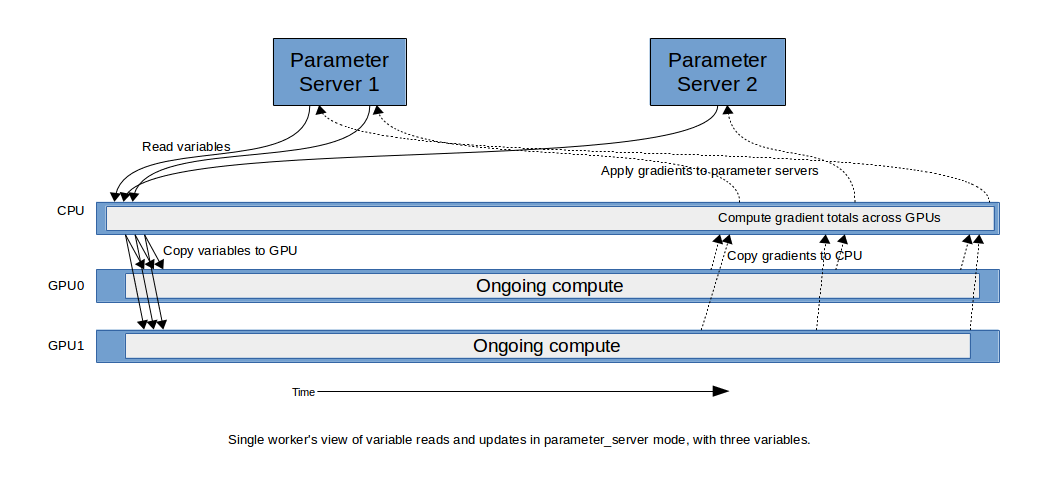
\includegraphics[scale=0.5]{perf_parameter_server_mode_doc.png}
\end{figure}
\subsection{复制的变量}
在这个设计中,每个在server上的GPU有自己的复制的变量。值通过应用完整的局和提取到每个GPU的复制变量保持同步。

变量和数据在训练开始的时候是可用的,因此钱想传递训练可以立即开始。梯度通过device聚合,完整的聚合的梯度是应用在每个本地复制。
梯度聚合通过server扩山到server有不同的方法:
\begin{itemize}
	\item 使用标准的TensorFlow操作聚合在一个单独的device(CPU或者GPU)然后复制它回到所有的GPUs
	\item 使用NVIDIANCCL,下面的NCCL章节描述。
\end{itemize}
这个模式可以通过传递--variable\_update=replicated用在脚本中。
\subsection{在分布式系统上训练时复制变量}
对于变量的复制方法可能被扩展到分布式训练。一个处理这样工作的方法是replicated mode:完全通过集群聚合梯度然后应用他们到每个本地复制变量。这在这个脚本的将来版本也许会显示,脚本呈现一个不同的变量,描述。

在这个模式,额外的每个GPU的复制变量,master的复制存储在村塾服务器。正如复制模式,训练可以用本地的复制的变量立即开始。

当权重的梯度可用的时候,他们送回参数服务器所有的本地复制被更新:
\begin{enumerate}
	\item 所有从同一个worker来的梯度被聚集在一起
	\item 从每个worker聚集的梯度被发送到参数服务器拥有的变量,这里制定的优化器用于更新master变量的复制
	\item 每个worker更新它从master复制的变量。在例程模型,这集合cross-replica做等待所有workers完成更新变量,仅仅在所有复制的障碍被释放后获取新的变量。当一个对所有变量的复制完成后,这标记训练的末端,下一步训练可以开始。
\end{enumerate}
尽管这听起来类似使用参数服务器的标准,但是性能进场更好。很可能是应为计算没有延迟,大量复制的梯度的时延可能通过之后的计算曾被隐
这个模式可以传递参数--variable\_update=distributed\_replicated用于脚本。
\begin{figure}[H]
	\centering
	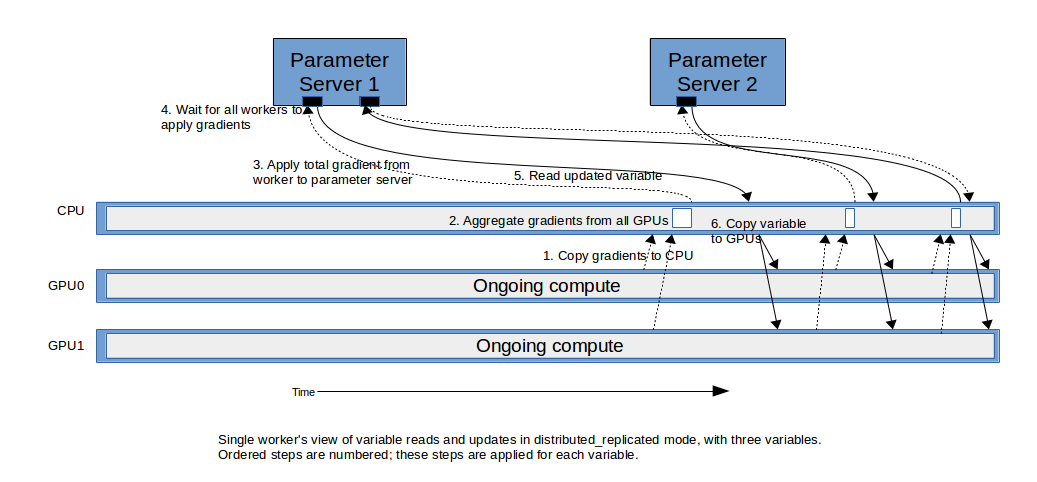
\includegraphics[scale=0.5]{perf_distributed_replicated_mode_doc.png}
\end{figure}
\subsection{NCCL}
为了广播变量在同一机器上通过不同的GPU聚合梯度梯度,我们可以使用默认的TensorFlow隐藏的复制机制。

然而,我们可以使用选项NCCL(\href{https://www.tensorflow.org/api_docs/python/tf/contrib/nccl}{tf.contrib.nccl})。NCCL是NVIDIA一个能在不同的GPU上可以高效广播和聚合数据库。它在每个GPU上调度一个cooperatting核心了解基础硬件拓扑下的最佳利用。这可信使用一个GPU的SM。

在我们的试验中,我们通过NCLL展示经常比本身有更快的数据聚合。我们的假设是隐含的复制隐含的基本的free因此他们能在GPU上复制引擎,只要时延能通过主要的计算本身隐藏。尽管NCLL可以更快的转换数据,接受一个SM,给基于L2cache添加更多压力。我们的结果显示8GPU,NCLL载入更好的性能。然而很少的GPU,隐含的复制性能更好。
\subsection{Staged变量}
我们进一步介绍一个staged变量模式,这里我们用staging area到变量读和他们的更新。类似输入pipeline的软件的pipelining,这可以隐藏数据复制时延。如果计算时间花费被复制和聚合更长,复制它本身变得essentially free。

缺点是所有的权重从之前训练步骤读取。因此它不同于SGD算法。但是它能通过掉着那个学习率和其它草参数可能改善收敛。

\subsection{执行脚本}
这个章节列出命令行参数的核心和有一些基本的执行主要脚本的例子( \href{https://github.com/tensorflow/benchmarks/tree/master/scripts/tf_cnn_benchmarks/tf_cnn_benchmarks.py}{tf\_cnn\_benchmarks.py})
\begin{quote}
	\textbf{注意:}\emph{tf\_cc\_benchmarks.py用在TensorFlow 1.1之后引入的force\_gpu\_campatible,知道TensorFlow 1.2被从源代码被释放被建议。}
\end{quote}
\subsection{基本的命令行参数}
\begin{itemize}
	\item model:模型使用。如resnet50,inception3,vgg16和alexnet
	\item num\_gpus:使用GPU的数量
	\item data\_dir:处理数据的路径。如果没有设置,中和数据被使用。用imagenet数据这些\href{https://github.com/tensorflow/models/tree/master/inception#getting-started}{说明}作为起点。
	\item batch\_size:每个GPU的批的尺寸
	\item variable\_update:管理变量的方法:parameter\_server ,replicated, distributed\_replicated, independent
	\item local\_parameter\_device:用作参数服务器的设备:CPU或者GPU
\end{itemize}
单个实例的例子
\begin{lstlisting}[language=Python]
# VGG16 training ImageNet with 8 GPUs using arguments that optimize for
# Google Compute Engine.
python tf_cnn_benchmarks.py --local_parameter_device=cpu --num_gpus=8 \
--batch_size=32 --model=vgg16 --data_dir=/home/ubuntu/imagenet/train \
--variable_update=parameter_server --nodistortions

# VGG16 training synthetic ImageNet data with 8 GPUs using arguments that
# optimize for the NVIDIA DGX-1.
python tf_cnn_benchmarks.py --local_parameter_device=gpu --num_gpus=8 \
--batch_size=64 --model=vgg16 --variable_update=replicated --use_nccl=True

# VGG16 training ImageNet data with 8 GPUs using arguments that optimize for
# Amazon EC2.
python tf_cnn_benchmarks.py --local_parameter_device=gpu --num_gpus=8 \
--batch_size=64 --model=vgg16 --variable_update=parameter_server

# ResNet-50 training ImageNet data with 8 GPUs using arguments that optimize for
# Amazon EC2.
python tf_cnn_benchmarks.py --local_parameter_device=gpu --num_gpus=8 \
--batch_size=64 --model=resnet50 --variable_update=replicated --use_nccl=False
\end{lstlisting}
\subsection{分布式的命令行参数}
\begin{itemize}
	\item ps\_host:逗号分隔的主机用作参数服务器,格式为<host>:port,例如10.0.0.2:50000
	\item worker\_hosts:逗号分隔的主机用作worker,格式<host>:port,例如10.0.0.2:50001
	\item task\_index:在ps\_hosts或者worker\_hosts开始的主机索引
	\item job\_name:输入job,例如ps或者worker 
\end{itemize}
\subsection{分布式的例子}
下面是一个在两台主机上训练ResNet-50的例子host\_0(10.0.0.1)和host\_1(10.0.0.2)使用中和数据的例子,用通过传递--data\_dir参数传递真实数据。
\begin{lstlisting}[language=Python]
# Run the following commands on host_0 (10.0.0.1):
python tf_cnn_benchmarks.py --local_parameter_device=gpu --num_gpus=8 \
--batch_size=64 --model=resnet50 --variable_update=distributed_replicated \
--job_name=worker --ps_hosts=10.0.0.1:50000,10.0.0.2:50000 \
--worker_hosts=10.0.0.1:50001,10.0.0.2:50001 --task_index=0

python tf_cnn_benchmarks.py --local_parameter_device=gpu --num_gpus=8 \
--batch_size=64 --model=resnet50 --variable_update=distributed_replicated \
--job_name=ps --ps_hosts=10.0.0.1:50000,10.0.0.2:50000 \
--worker_hosts=10.0.0.1:50001,10.0.0.2:50001 --task_index=0

# Run the following commands on host_1 (10.0.0.2):
python tf_cnn_benchmarks.py --local_parameter_device=gpu --num_gpus=8 \
--batch_size=64 --model=resnet50 --variable_update=distributed_replicated \
--job_name=worker --ps_hosts=10.0.0.1:50000,10.0.0.2:50000 \
--worker_hosts=10.0.0.1:50001,10.0.0.2:50001 --task_index=1

python tf_cnn_benchmarks.py --local_parameter_device=gpu --num_gpus=8 \
--batch_size=64 --model=resnet50 --variable_update=distributed_replicated \
--job_name=ps --ps_hosts=10.0.0.1:50000,10.0.0.2:50000 \
--worker_hosts=10.0.0.1:50001,10.0.0.2:50001 --task_index=1
\end{lstlisting}
\section{基准测试}
\subsection{概览}
选择的图像分类模型被多平台测试为TensorFlow社区创建一个参考点。在\href{https://www.tensorflow.org/performance/benchmarks#methodology}{Methodology }章节详细描述了测试如何执行和连接到使用脚本。
\subsection{图形分类模型的结果}
InceptionV3(\href{https://arxiv.org/abs/1512.00567}{arXiv:1512.00567)}),ResNet-50(\href{https://arxiv.org/abs/1512.03385}{arXiv:1512.03385}),ResNet-152(\href{https://arxiv.org/abs/1512.03385}{arXiv:1512.03385}),VGG16(\href{https://arxiv.org/abs/1409.1556}{arXiv:1409.1556})和\href{http://papers.nips.cc/paper/4824-imagenet-classification-with-deep-convolutional-neural-networks.pdf}{AlexNet}使用\href{http://www.image-net.org/}{ImageNet}数据集。测试运行在Google Compute Engine,Amazon Elastic Compute Cloud(Amazon EC2),和NVIDIA DGX-1。多数测试运行在合成和真实数据上。测试合成数据通过使用tf.Variable设置相同的形状作为ImageNet模型的数据期望。我们相信在一个平台的基准测试上它是很有用的。这载入基础的永健和实际训练准备数据的框架测试。我们结合合成数据移除磁盘I/O作为变量设置baseline。真真的数据用于验证TensorFlow输入pipeline和基础的磁盘I/O在计算单元上是饱和。
\subsection{在NVIDIA DGX-1(NVIDIA Tesla P100)}
\begin{figure}[H]
	\centering
	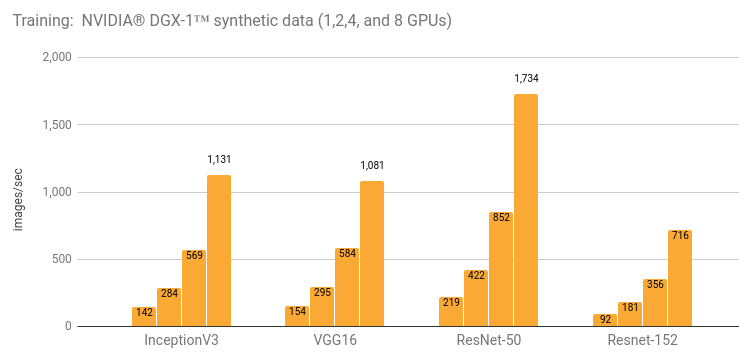
\includegraphics[scale=0.5]{perf_summary_p100_single_server.png}
\end{figure}
详细的额外的结果在\href{https://www.tensorflow.org/performance/benchmarks#details_for_nvidia_dgx-1tm_nvidia_tesla_p100}{Details for NVIDIA® DGX-1 (NVIDIA TeslaP100)}
\begin{figure}[H]
	\centering
	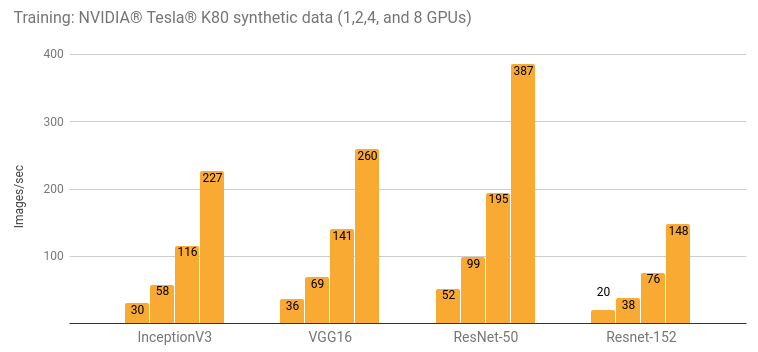
\includegraphics[scale=0.5]{perf_summary_k80_single_server.png}
\end{figure}
详细的额外的结果在\href{https://www.tensorflow.org/performance/benchmarks#details_for_google_compute_engine_nvidia_tesla_k80}{Details for Google Compute Engine (NVIDIA Tesla K80) }和\href{https://www.tensorflow.org/performance/benchmarks#details_for_amazon_ec2_nvidia_tesla_k80}{ Details for Amazon EC2 (NVIDIA Tesla K80) }
\subsection{用Tesla K80分布式的训练}
\begin{figure}[H]
	\centering
	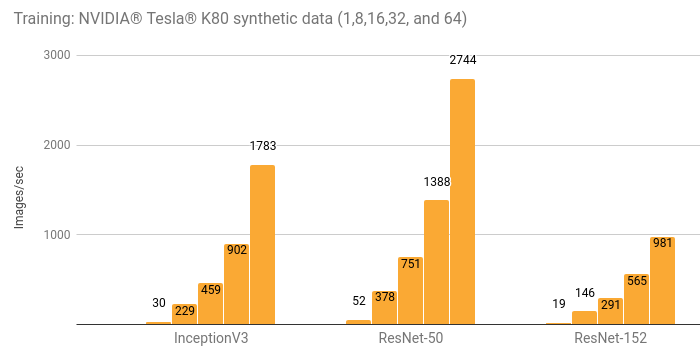
\includegraphics[scale=0.5]{perf_summary_k80_aws_distributed.png}
\end{figure}
详细的信息在\nameref{subsec:1}
\subsection{结合真是数据训练比较}
\centering
\begin{figure}[H]
	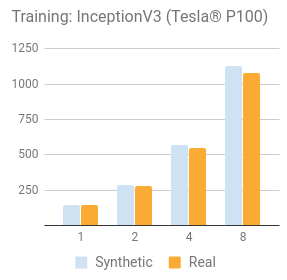
\includegraphics[scale=0.5]{perf_summary_p100_data_compare_inceptionv3}
	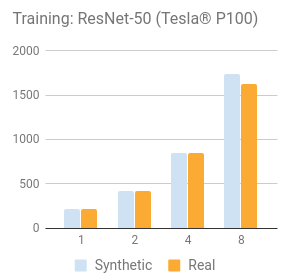
\includegraphics[scale=0.5]{perf_summary_p100_data_compare_resnet50}
\end{figure}
NVIDIA Tesla K80
\begin{figure}[H]
	\centering
	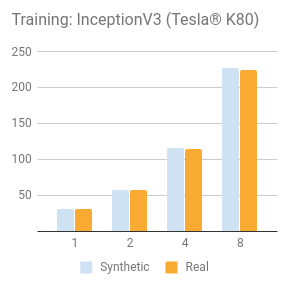
\includegraphics[scale=0.5]{perf_summary_k80_data_compare_inceptionv3.png}
	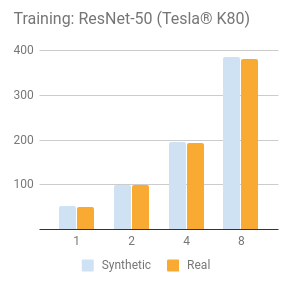
\includegraphics[scale=0.5]{perf_summary_k80_data_compare_resnet50.png}
\end{figure}
\subsection{详细的NVIDIA DGX-1(NVIDIA Tesla P100)}
\textbf{环境}\newline
\begin{itemize}
	\item 实例类型:NVIDIA DGX-1
	\item GPU:8x NVIDIA Tesla P100
	\item OS:通过Docker特使运行Ubuntu 16.0.4 LTS 
	\item CUDA/cuDNN"8.0/5.1
	\item TensorFlow GitHub b1e174e
	\item Benchmark GitHub hash:9165a70
	\item 构建命令:\lstinline[language=Bash]{bazel build -c opt --copt=-march="haswell" --config=cuda //tensorflow/tools/pip_package:build_pip_package}
	\item Disk:本地SSD
	\item Dataset:ImageNet
	\item Test Data:2017五月
\end{itemize}
用于模型的批大小和优化器在下表。另外在表中的批大小,Inception V3,ResNet-50,ResNet152和VGG16用于在批大小为32上测试,这些值在其他的结果章节:
\begin{table}[H]
	\centering
	\begin{tabular}{|c|c|c|c|c|c|}
		\hline
		选项&Inception v3&ResNet-50&ResNet-152&AlexNet&VGG16\\
		\hline
		每个GPU批的大小&64&64&64&512&64\\
		\hline
		优化器&sgd&sgd&sgd&sgd&sgd\\
		\hline
	\end{tabular}
\end{table}
为每个模型配置:
\begin{table}[H]
	\centering
	\begin{tabular}{|c|c|c|}
		\hline
	模型&变量更新&本地变量设备\\
		\hline
		InceptionV3 &参数服务器&cpu\\
		\hline
		ResNet50 &参数服务器&cpu\\
		\hline
		ResNet152 &参数服务器&cpu\\
		\hline
		AlexNet &参数服务器&cpu\\
		\hline
		VGG16 &参数服务器&cpu\\
		\hline
	\end{tabular}
\end{table}
结果:
\begin{figure}[H]
	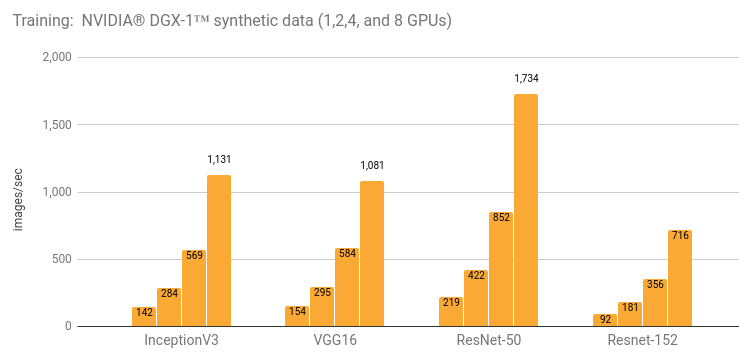
\includegraphics[scale=0.5]{perf_summary_p100_single_server.png}
	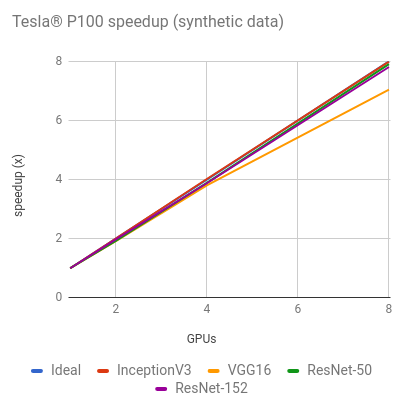
\includegraphics[scale=0.5]{perf_dgx1_synth_p100_single_server_scaling.png}
\end{figure}
训练聚合数据
\begin{table}[H]
	\centering
	\begin{tabular}{|c|c|c|c|c|c|}
		\hline
		GPUs	&InceptionV3	&ResNet-50	&ResNet-152	&AlexNet	&VGG16\\
		\hline
		1	&142	&219	&91.8	&2987	&154\\
		\hline
		2	&284	&422	&181	&5658	&295\\
		\hline
		4	&569	&852	&356	&10509	&584\\
		\hline
		8	&1131	&1734	&716	&17822	&1081\\
		\hline
	\end{tabular}
\end{table}
训练真是数据
\begin{table}[H]
	\centering
	\begin{tabular}{|c|c|c|c|c|c|}
		\hline
		GPUs	&InceptionV3	&ResNet-50	&ResNet-152	&AlexNet	&VGG16\\
		\hline
		1	&142	&218	&91.4	&2890	&154\\
		\hline
		2	&278	&425	&179	&4448	&284\\
		\hline
		4	&551	&853	&359	&7105	&534\\
		\hline
		8	&1079	&1630	&708	&N/A	&898\\
		\hline
	\end{tabular}
\end{table}
在8GPUs结合真实数据训练AlexNet从图上包含上面的表格最大化输入pipeline。
其他的结果

下面的结果每批32
\textbf{训练综合数据}
\begin{table}[H]
	\centering
	\begin{tabular}{|c|c|c|c|c|}
		\hline
		GPUs	&InceptionV3	&ResNet-50	&ResNet-152	&VGG16\\
		\hline
		1	&128	&195	&82.7	&144\\
		\hline
		2	&259	&368	&160	&281\\
		\hline
		4	&520	&768	&317	&549\\
		\hline
		8	&995	&1485	&632	&820\\
		\hline
	\end{tabular}
\end{table}

训练真实数据
\begin{table}
	\centering
	\begin{tabular}{|c|c|c|c|c|}
		\hline
		GPUs	&InceptionV3	&ResNet-50	&ResNet-152	&VGG16\\
		\hline
		1	&130	&193	&82.4	&144\\
		\hline
		2	&257	&369	&159	&253\\
		\hline
		4	&507	&760	&317	&457\\
		\hline
		8	&966	&1410	&609	&690\\
		\hline
	\end{tabular}
\end{table}
在Google Compute Engine上详情(NVIDIA Tesla K80)
\begin{itemize}
	\item  实例类型:n1-standard-32-k80x8
	\item  GPU:8 NVIDIA Tesla K80
	\item OS Ubuntu 16.04 LTS 
	\item CUDA/cuDNN:8.0/5.1
	\item TensorFlow GitHub hash:b1e174e
	\item Benchmark Github hash:9165a70
	\item 构建命令\lstinline[language=Bash]{bazel build -c opt --copt=-march="haswell" --config=cuda //tensorflow/tools/pip_package:build_pip_package}
	\item Disk:1.7TB共享SSD永久磁盘
	\item Dataset:ImageNet 
	\item Test Data:2017 5月
\end{itemize}
每个模型的批大小和优化器在下表中。另外批大小列在表格,InceptionV3和ResNet-50被测试一个batch为32,这些结果在其他章节。
\begin{table}[H]
	\centering
	\begin{tabular}{|c|c|c|c|c|c|}
		\hline
		Options	&InceptionV3	&ResNet-50	&ResNet-152	&AlexNet	&VGG16\\
		\hline
		Batch size per GPU	&64	&64	&32	&512	&32\\
		\hline
		Optimizer	&sgd	&sgd	&sgd	&sgd	&sgd\\
		\hline
	\end{tabular}
\end{table}
这配置用于每个模型variable\_update等于parameter\_server和local\_parameter\_device等于cpu。
\textbf{结果}\\
\begin{figure}[H]
	\centering
	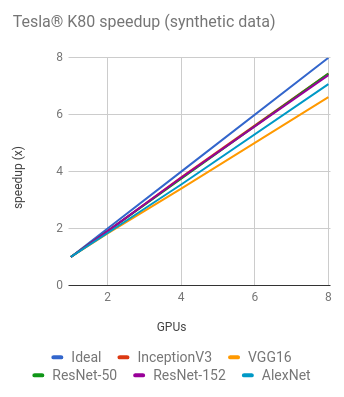
\includegraphics[scale=0.5]{perf_gce_synth_k80_single_server_scaling.png}
	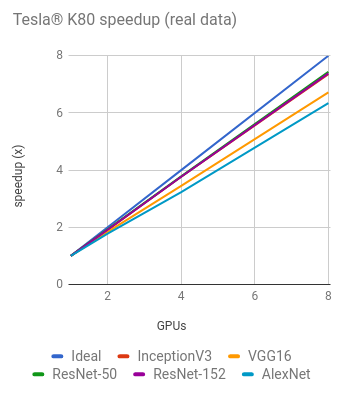
\includegraphics[scale=0.5]{perf_gce_real_k80_single_server_scaling.png}
\end{figure}
\begin{table}[H]
	\centering
	\begin{tabular}{|c|c|c|c|c|c|}
		\hline
		GPUs	&InceptionV3	&ResNet-50	&ResNet-152	&AlexNet	&VGG16\\
		\hline
		1	&30.5	&51.9	&20.0	&656	&35.4\\
		\hline
		2	&57.8	&99.0	&38.2	&1209	&64.8\\
		\hline
		4	&116	&195	&75.8	&2328	&120\\
		\hline
		8	&227	&387	&148	&4640	&234\\
		\hline
	\end{tabular}
	\caption{Training synthetic data}
\end{table}
\begin{table}[H]
	\centering
	\begin{tabular}{|c|c|c|c|c|c|}
		\hline
		GPUs	&InceptionV3	&ResNet-50	&ResNet-152	&AlexNet	&VGG16\\
		\hline
		1	&30.6	&51.2	&20.0	&639	&34.2\\
		\hline
		2	&58.4	&98.8	&38.3	&1136	&62.9\\
		\hline
		4	&115	&194	&75.4	&2067	&118\\
		\hline
		8	&225	&381	&148	&4056	&230\\
		\hline
	\end{tabular}
	\caption{训练真实数据}
\end{table}
\begin{table}[H]
	\centering
	\begin{tabular}{|c|c|c|}
		\hline
		GPUs	&InceptionV3 (batch size 32)	&ResNet-50 (batch size 32)\\
		\hline
		1	&29.3	&49.5\\
		\hline
		2	&55.0	&95.4\\
		\hline
		4	&109	&183\\
		\hline
		8	&216	&362\\
		\hline
	\end{tabular}
	\caption{Training real data}
\end{table}
\subsection{Amazon Ec2详情(NVIDIA Tesla K80)}
环境
\begin{itemize}
	\item 实例类型:p2.8xlarge
	\item GPU:8x NVIDIA Tesla K80
	\item OS:Ubuntu16.0.4 LTS 
	\item CUDA/cuDNN:8.0/5.1
	\item TensorFlow Github hash:b1e174e
	\item Benchmark GitHub hash:9165a70
	\item 构建命令\lstinline[language=Bash]{bazel build -c opt --copt=-march="haswell" --config=cuda //tensorflow/tools/pip_package:build_pip_package}
	\item Disk:1TB Amazon EFS(brush 100MiB/sec for 12 hours,continous 50 MiB/sec)
	\item Dataset:ImageNet 
	\item TestData:2017 5月
\end{itemize}
用于每个模型的Batch size和优化器在下表。另外batch size列出在表格中,InceptionV3和ResNet-50用于在batch为32上测试。这些结果在其它章节
\begin{table}[!h]
	\centering
\begin{tabular}{|c|c|c|c|c|c|}
		\hline
	Options	InceptionV3	&InceptionV3    &ResNet-50	&ResNet-152	&AlexNet	&VGG16\\
		\hline
	Batch size per GPU	&64	&64	&32	&512	&32\\
		\hline
	Optimizer	&sgd	&sgd	&sgd	&sgd	&sgd\\
		\hline
\end{tabular}
\end{table}
用于每个模型的配置
\begin{table}[H]
	\centering
	\begin{tabular}{|c|c|c|}
		\hline
		Model	&variable\_update	&local\_parameter\_device\\
		\hline
		InceptionV3	&parameter\_server	&cpu\\
		\hline
		ResNet-50	&replicated (without NCCL)	&gpu\\
		\hline
		ResNet-152	&replicated (without NCCL)	&gpu\\
		\hline
		AlexNet	&parameter\_server	&gpu\\
		\hline
		VGG16	&parameter\_server	&GPUs \\
		\hline
	\end{tabular}
\end{table}
 结果
 \begin{figure}[H]
	 \centering
	 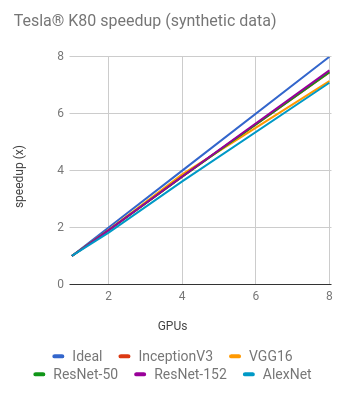
\includegraphics[scale=0.5]{perf_aws_synth_k80_single_server_scaling.png}
	 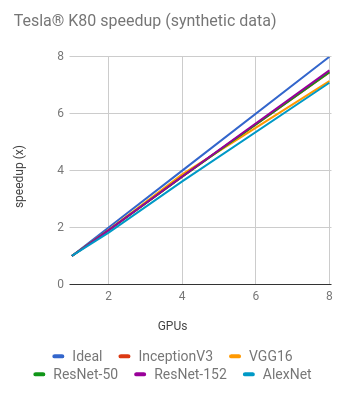
\includegraphics[scale=0.5]{perf_aws_synth_k80_single_server_scaling.png}
 \end{figure}
 \begin{table}[H]
	\centering
	\begin{tabular}{|c|c|c|c|c|c|}
		\hline
		GPUs	&InceptionV3	&ResNet-50	&ResNet-152	&AlexNet	&VGG16\\
		\hline
		1	&30.8	&51.5	&19.7	&684	&36.3\\
		\hline
		2	&58.7	&98.0	&37.6	&1244	&69.4\\
		\hline
		4	&117	&195	&74.9	&2479	&141\\
		\hline
		8	&230	&384	&149	&4853	&260\\
		\hline
	\end{tabular}
	 \caption{Training synthetic data}
\end{table}
 \begin{table}[H]
	 \centering
	 \begin{tabular}{|c|c|c|c|c|c|}
		\hline
		 GPUs	&InceptionV3	&ResNet-50	&ResNet-152	&AlexNet	&VGG16\\
		\hline
		 1	&30.5	&51.3	&19.7	&674	&36.3\\
		\hline
		 2	&59.0	&94.9	&38.2	&1227	&67.5\\
		\hline
		 4	&118	&188	&75.2	&2201	&136\\
		\hline
		 8	&228	&373	&149	&N/A	&242\\
		\hline
	 \end{tabular}
 \end{table}
 结合8GPU从图上和表格训练真实数据因为我们的RFS设置没有提供足够的吞吐量。
 
 其他的结果
 \begin{table}[H]
	\centering
	\begin{tabular}{|c|c|c|}
		\hline
		GPUs	&InceptionV3 (batch size 32)	&ResNet-50 (batch size 32)\\
		\hline
		1	&29.9	&49.0\\
		\hline
		2	&57.5	&94.1\\
		\hline
		4	&114	&184\\
		\hline
		8	&216	&355\\
		\hline
	\end{tabular}
	 \caption{Training synthetic data}
\end{table}
 \begin{table}[H]
	\centering
	\begin{tabular}{|c|c|c|}
		\hline
		GPUs	&InceptionV3 (batch size 32)	&ResNet-50 (batch size 32)\\
		\hline
		1	&30.0	&49.1\\
		\hline
		2	&57.5	&95.1\\
		\hline
		4	&113	&185\\
		\hline
		8	&212	&353\\
		\hline
	\end{tabular}
	 \caption{Training real data}
\end{table}
 \subsection{在Amazon EC2上(NVIDIA Tesla K80)}
 \begin{itemize}
	 \item Instance type: p2.8xlarge
         \item GPU: 8x NVIDIA® Tesla® K80
	 \item  OS: Ubuntu 16.04 LTS
	\item 	 CUDA / cuDNN: 8.0 / 5.1
	\item 	 TensorFlow GitHub hash: b1e174e
	\item 	 Benchmark GitHub hash: 9165a70
	\item 	\lstinline[language=Bash]{ Build Command: bazel build -c opt --copt=-march="haswell" --config=cuda //tensorflow/tools/pip_package:build_pip_package}
	\item 	 Disk: 1.0 TB EFS (burst 100 MB/sec for 12 hours, continuous 50 MB/sec)
	\item 	 DataSet: ImageNet
	\item	 Test Date: May 2017
 \end{itemize}
 用于测试的批和优化器在下表。另外批大小在表格中,InceptionV3和ResNet-50用于在批大小为32上测试。这结果在其它章节。
 \begin{table}[H]
	\centering
	 \begin{tabular}{|c|c|c|c|}
		\hline
		 Options	&InceptionV3	&ResNet-50	&ResNet-152\\
		\hline
		 Batch size per GPU	&64	&64	&32\\
		\hline
		 Optimizer	&sgd	&sgd	&sgd\\
		\hline

	 \end{tabular}
 \end{table}
 用于每个模型的配置

\begin{table}
	\centering
	\begin{tabular}{|c|c|c|c|}
		\hline
		Model	&variable\_update	&local\_parameter\_device	&cross\_replica\_sync\\
		\hline
		InceptionV3	&distributed\_replicated	&n/a	&True\\
		\hline
		ResNet-50	&distributed\_replicated	&n/a	&True\\
		\hline
		ResNet-152	&distributed\_replicated	&n/a	&True\\
		\hline
	\end{tabular}
\end{table}
为了简化服务器设置,EC2实例(p2.8xlarge)运行在worker服务器上也运行在参数服务器上。参数服务器数量和worker服务器用:
\begin{itemize}
		\item InceptionV3:8实例/参数服务器
		\item ResNet50:(批大小为32)8实例/4参数服务器
		\item ResNet-152:8shili /4参数服务器
\end{itemize}
 结果
 \begin{figure}[H]
	 \centering
	 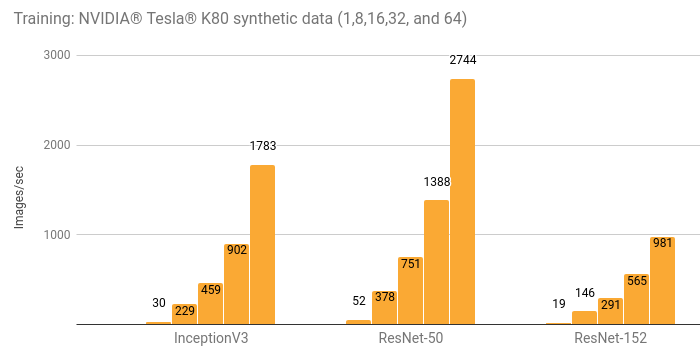
\includegraphics[scale=0.5]{perf_summary_k80_aws_distributed.png}
 \end{figure}
 \begin{figure}[H]
	 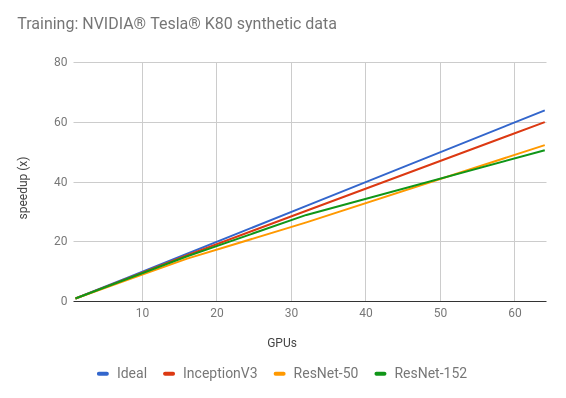
\includegraphics[scale=0.5]{perf_aws_synth_k80_distributed_scaling.png}
 \end{figure}
 \begin{table}
	\centering
	 \begin{tabular}{|c|c|c|c|}
		\hline
		 GPUs	&InceptionV3	&ResNet-50	&ResNet-152\\
		\hline
		 1	&29.7	&52.4	&19.4\\
		\hline
		 8	&229	&378	&146\\
		\hline
		 16	&459	&751	&291\\
		\hline
		 32	&902	&1388	&565\\
		\hline
		 64	&1783	&2744	&981\\
		\hline
	 \end{tabular}
 \end{table}
 其他结果
 \begin{figure}[H]
	 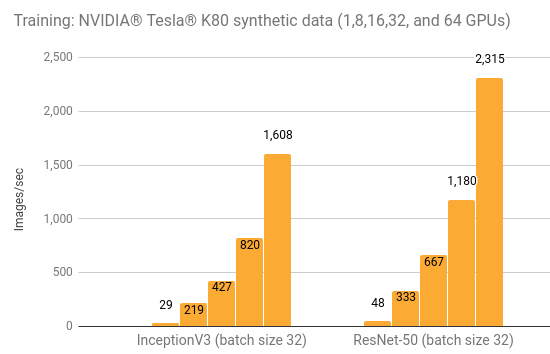
\includegraphics[scale=0.5]{perf_aws_synth_k80_multi_server_batch32.png}
 \end{figure}
 \begin{table}[H]
	\centering
	 \begin{tabular}{|c|c|c|}
		\hline
		 GPUs	&InceptionV3 (batch size 32)	&ResNet-50 (batch size 32)\\
		\hline
		 1	&29.2	&48.4\\
		\hline
		 8	&219	&333\\
		\hline
		 16	&427	&667\\
		\hline
		 32	&820	&1180\\
		\hline
		 64	&1608	&2315\\
		\hline
	 \end{tabular}
 \end{table}
 \subsection{方法论}
 这个\href{https://github.com/tensorflow/benchmarks/tree/master/scripts/tf_cnn_benchmarks}{脚本}运行在多个平台生成上面的结果。\href{https://www.tensorflow.org/performance/performance_models}{High-Performance Models}如何执行脚本的例子的详细技术在脚本中。

 为了创建结果可重复,没个测试运行5次然后时间被平均。GPU运行在默认给定的平台。对于NVIDIA Tesla K80这意味着让\href{https://devblogs.nvidia.com/parallelforall/increase-performance-gpu-boost-k80-autoboost/}{GPU Boose},10warmup步被做然后下一个100步被平均。













